\section{Struktur}

\paragraph{Event Sourcing} består af en sekvens af events, som er gemt i en Event Store af et eller anden format (SQL, noSQL, etc.), og bliver som regel brugt som en log, hvor i klasser kan se historiken af objekter, via. events. 

\begin{figure}[H]
    \centering
    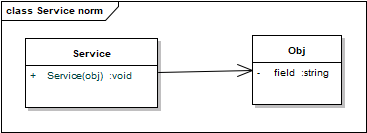
\includegraphics[width=0.7\linewidth]{Service-norm.png}
    \captionof{figure}{Simpel service model}
    \label{fig:service-model}
\end{figure}

På figur \ref{fig:service-model}, er der en simpel service, der gør et eller andet med et objekt, hvad den gør er underordnet, men den påvirker Obj på en eller anden måde. I et system uden Event Sourcing, vil det tidligere stadie af objektet være destrueret og glemt.

\begin{figure}[H]
    \centering
    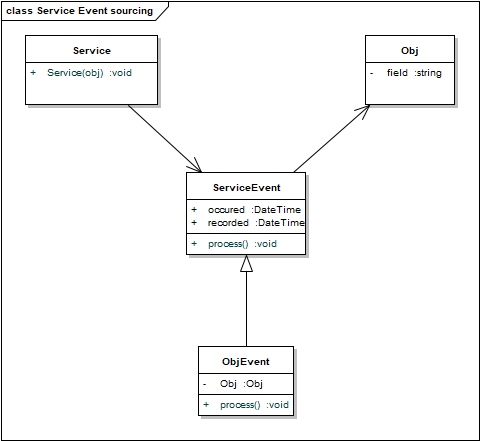
\includegraphics[width=0.7\linewidth]{Service-ES.png}
    \captionof{figure}{Simpel service med Event sourcing}
    \label{fig:service-ES-model}
\end{figure}

På figur \ref{fig:service-ES-model} er der introduceret et event med et ServiceEvent, som kan bruges til at gemme stadiet af denne handling. Selve funktionaliten er ikke ændret, men Handlingen kan nu persistesteres. 